\documentclass{article}
\usepackage{fancyhdr}
\pagestyle {fancy}
\title{3D Doctor}
\title{\textbf{3D DOCTOR}}
\author{MD: SHIHAB HOSSAIN}
\usepackage{graphicx}
\begin{document}
\pagenumbering{arabic}
\maketitle
\section{Author Details }
\begin{LARGE}
\begin{flushleft}
\textbf{E-mail: shihab.hossain5239@gmail.com}\\
\end{flushleft}
\begin{flushleft}
\textbf{STUDENT ID: 18ICTCSE038}\\
\end{flushleft}
\date\textbf{\today}
\end{LARGE}
\subsubsection{picture add}
\noindent
\begin{figure}[h]
\centering
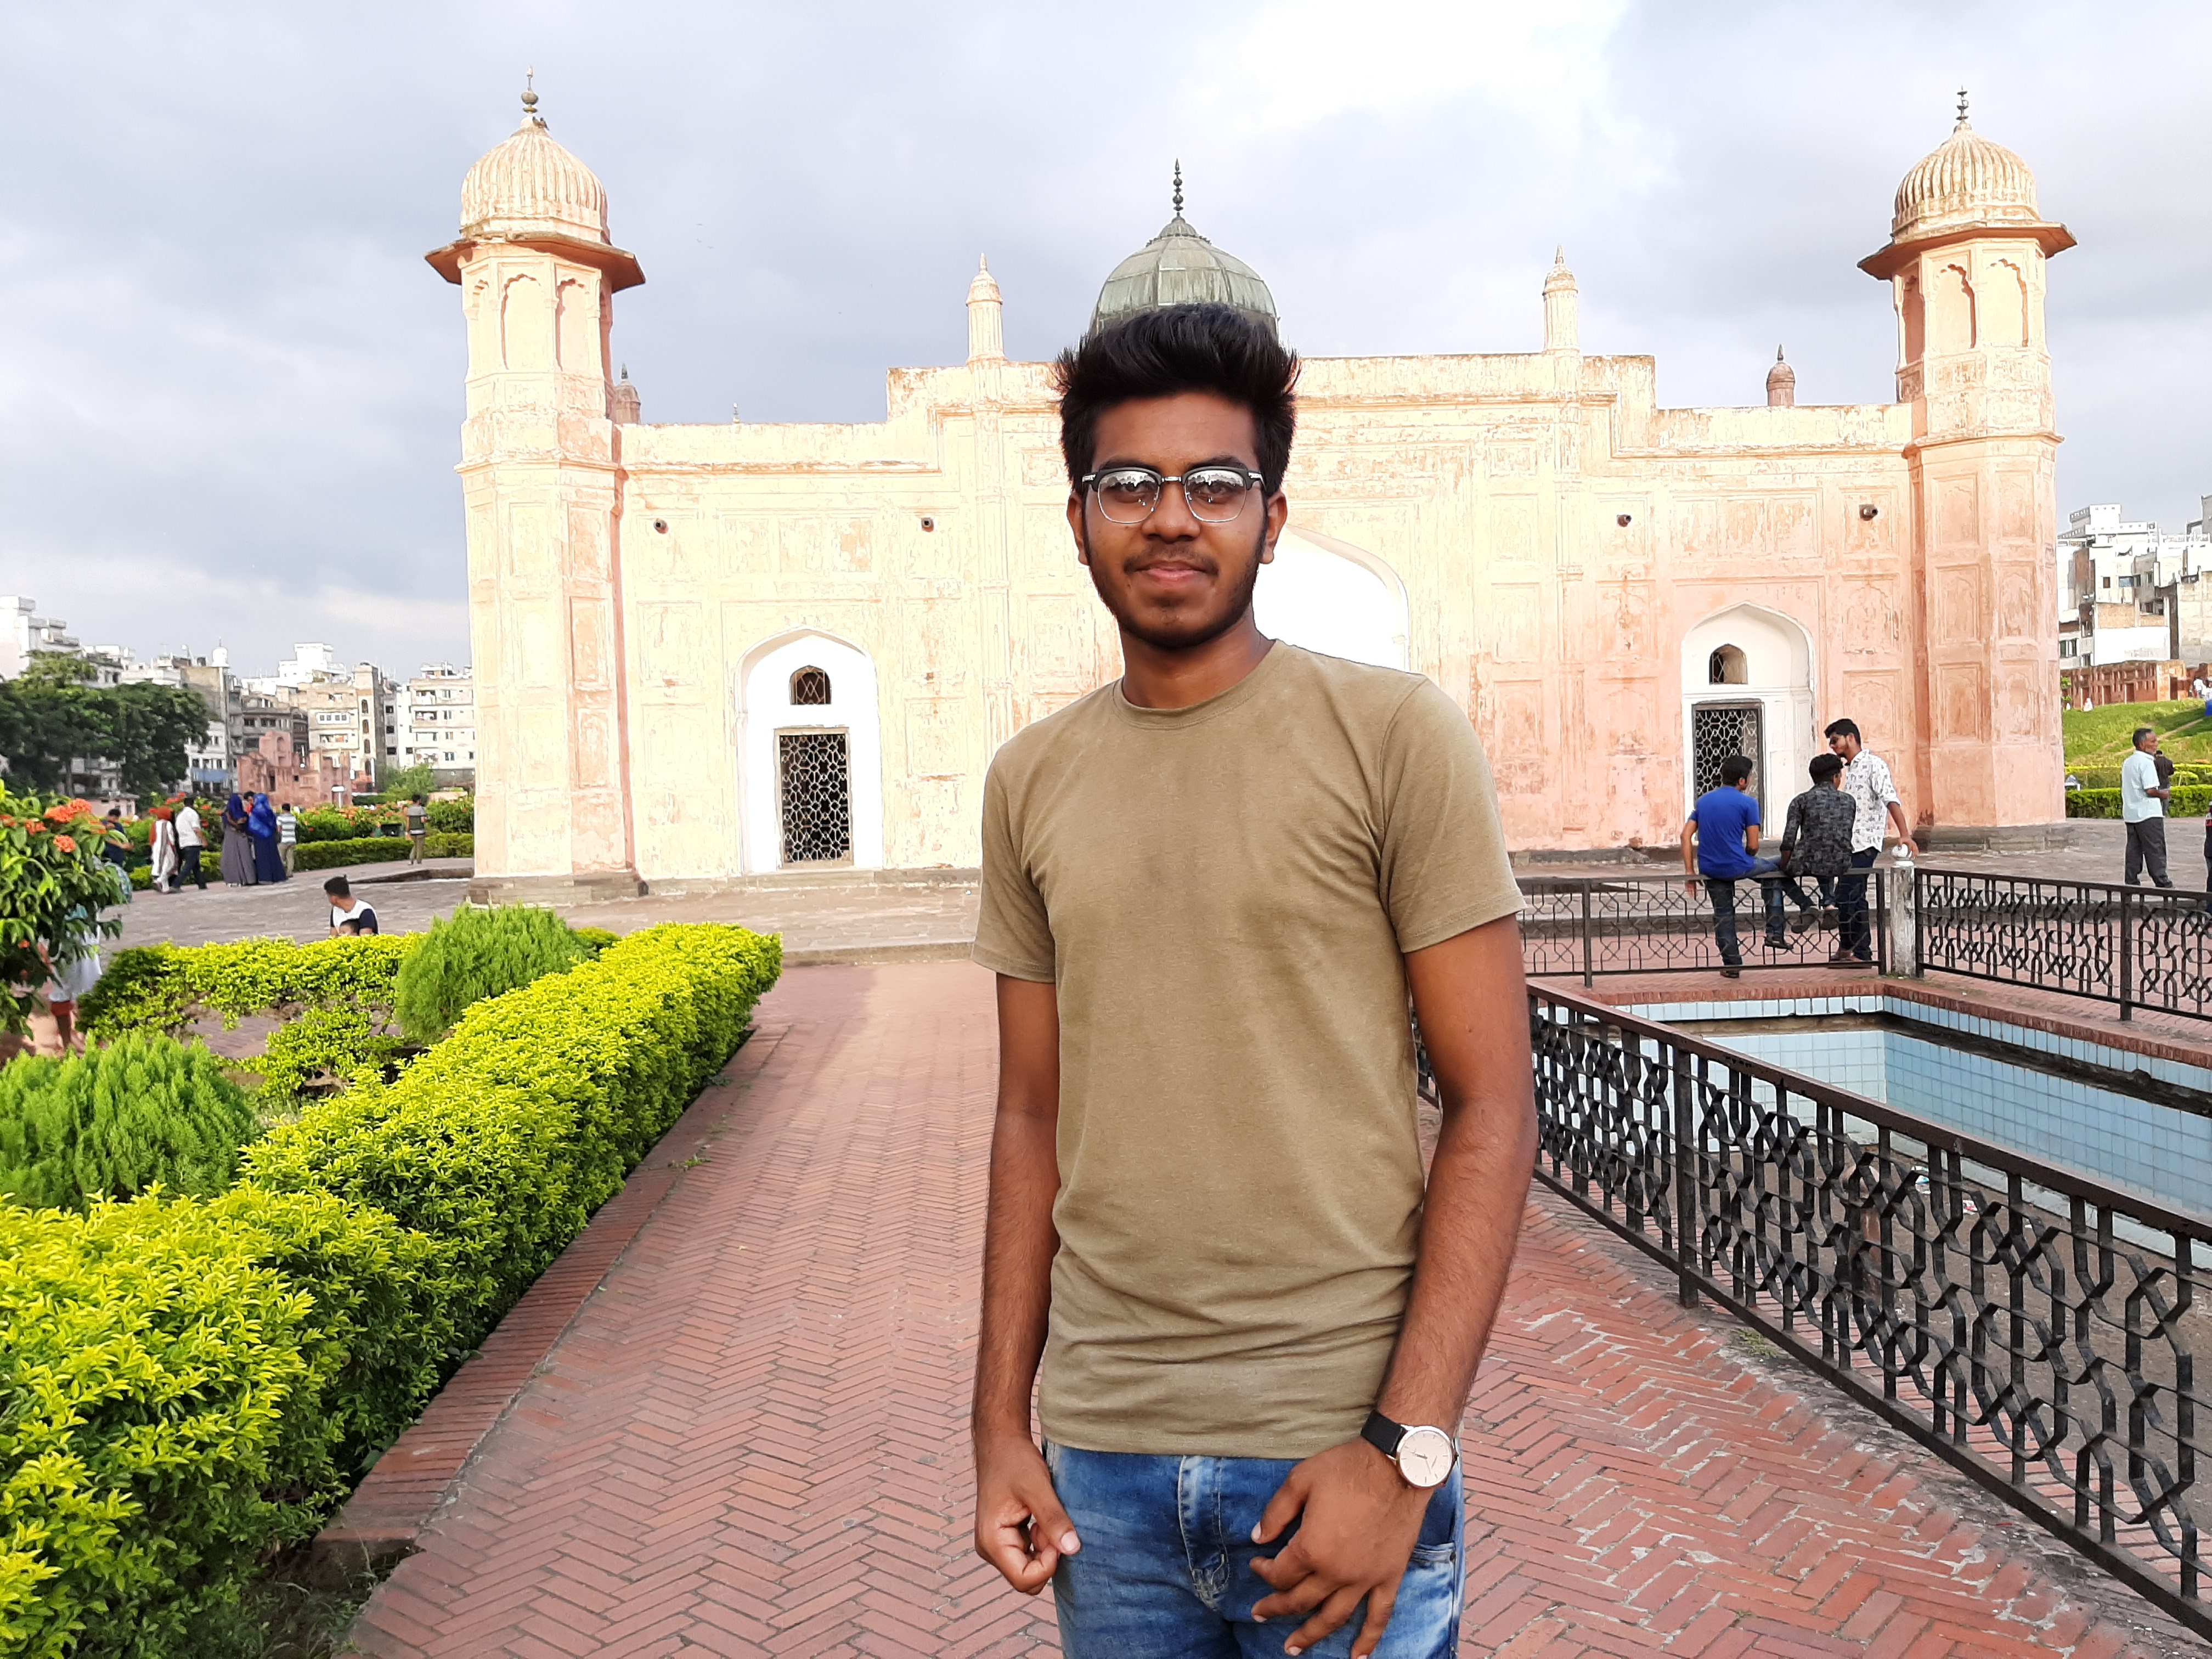
\includegraphics[width=200px,height=200px]{k.jpg}
\caption{Author}
\label{shihab}
\end{figure}
\newpage
\maketitle
\begin{huge}
\begin{center}
\textit{Introduction}
\end{center}
\end{huge}
\tableofcontents
\newpage
\section{Introduction}
\section{\textbf{What is 3D DOCTOR ?}}
"3D-DOCTOR Software has been one of the tremendous analysis software that I use on a regular bases to extract information from image files to create 3D model.
\subsection{About 3D Doctor}
3D-DOCTOR supports both grayscale and color images stored in DICOM, TIFF, Interfile, GIF, JPEG, PNG, BMP, PGM, MRC, RAW or other image file formats. 3D-DOCTOR creates 3D surface models and volume rendering from 2D cross-section images in real time on your PC.
\\
\begin{figure}[h]
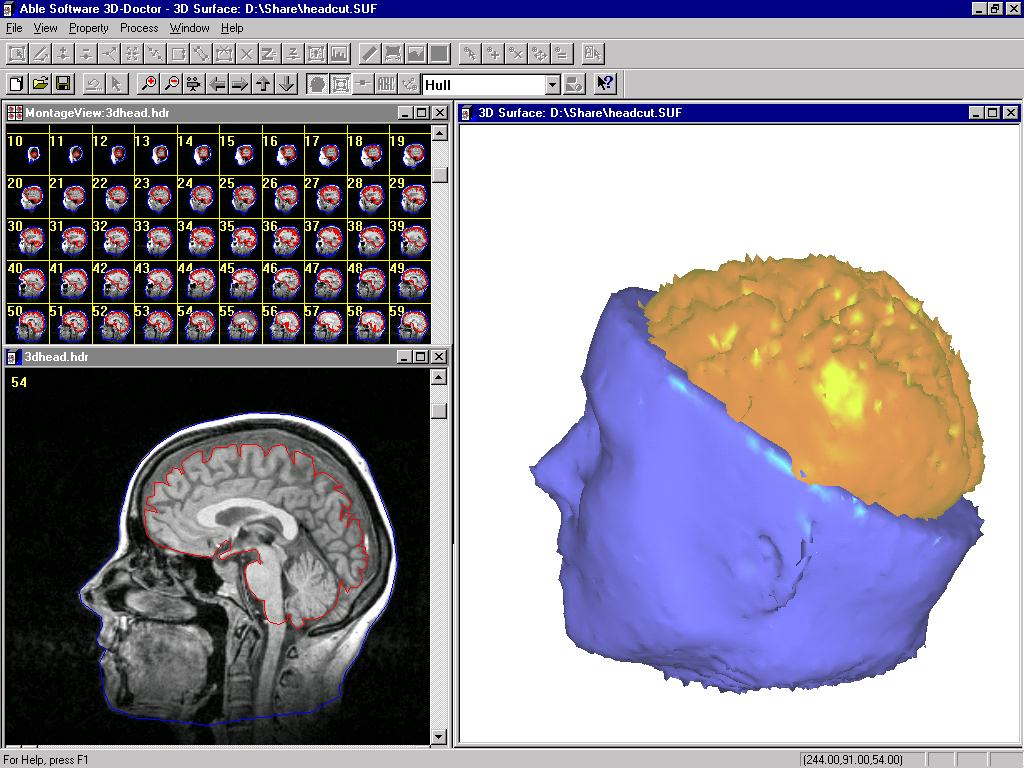
\includegraphics[width=300px,height=200px]{c.jpg}
\caption{image of 3D}
\label{shihab}
\end{figure}
\\
\newpage
\subsection{How it works?}
You can export the polygonal mesh models to STL (ASCII and Binary), DXF, IGES, 3DS, OBJ, VRML, PLY,  XYZ and other formats for surgical planning, simulation, quantitative analysis, finite element analysis (FEA) and rapid prototyping applications. You can calculate 3D volume and make other 3D measurements for quantitative analysis. 3D-DOCTOR's vector-based tools support easy image data handling, measurement, and analysis. 
\\
\begin{figure}[h]
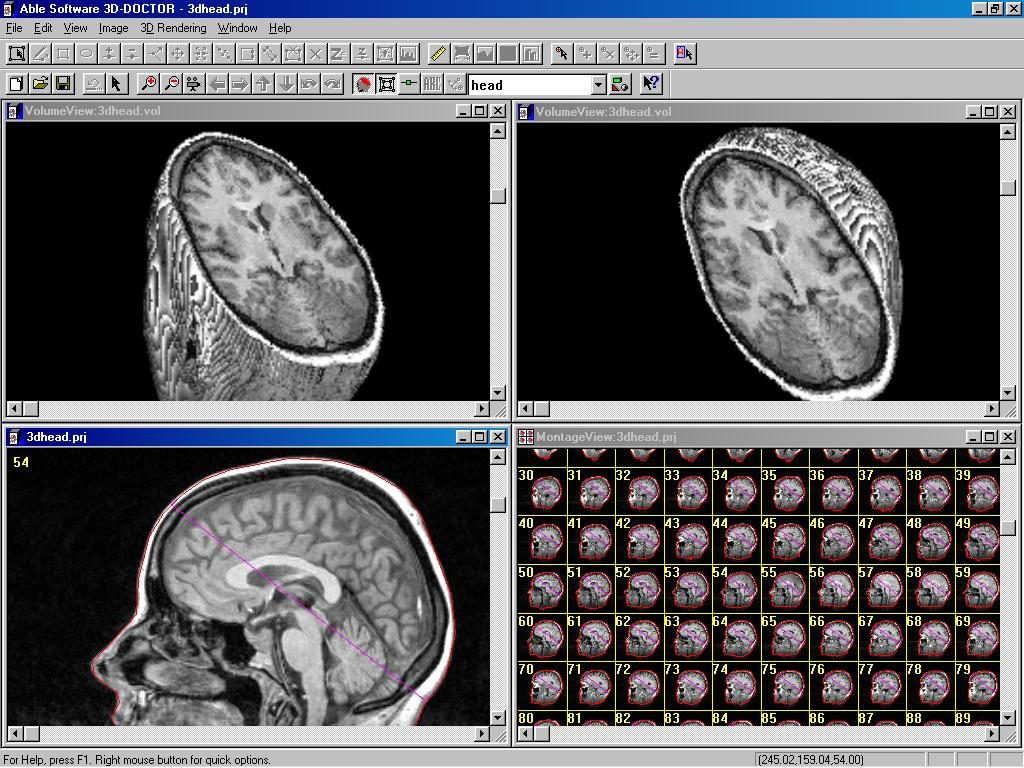
\includegraphics[width=300px,height=300px]{d.jpg}
\caption{image of 3D}
\label{picture}
\end{figure}
\newpage
\section{\begin{LARGE}
Applications of 3D Doctor
\end{LARGE}}
\begin{itemize}
\item
Bone Modeling From CT  Scan
\item
Modeling Soft Tissue From MRI

\item Volume Calculation
\item
Rapid Prototyping and 3D Printing
\item
Volume Rendering 
\item
Jaw Modeling From Dental CT
\item 
Registration and Fusion 
\item
Microscopy Imaging 
\end{itemize}
\newpage
\section{Bone Modeling From CT  Scan}
\subsection{How it works }
Computed tomography (CT) is an imaging technique that uses special x-ray equipment to obtain cross-sectional images of the body. A CT image normally has different pixel intensity range for tissues such as bones, organs and other tissues. The threshold-based "Interactive Segmentation" provides an easy way to segment a CT image for 3D modeling.

A 3D mesh model can be created from a CT image in 3 main steps:

Step 1. Open the CT image. If the image slices come in as separate files, use the "New Stack" command. 

Step 2. Use the "Interactive Segmentation" to generate object boundaries. For small size soft tissues, the manual tracing method can also be used. Boundaries can be edited using the boundary editor.

Step 3. Create 3D mesh models using the surface rendering command. The models can be exported to STL (ASCII and Binary), DXF, VRML, 3DS, OBJ, PLY  and other formats for 3D measurement, rapid prototyping, simulation, treatment planning and other applications.
\subsection{Multiple image addition}
\begin{figure}[h]
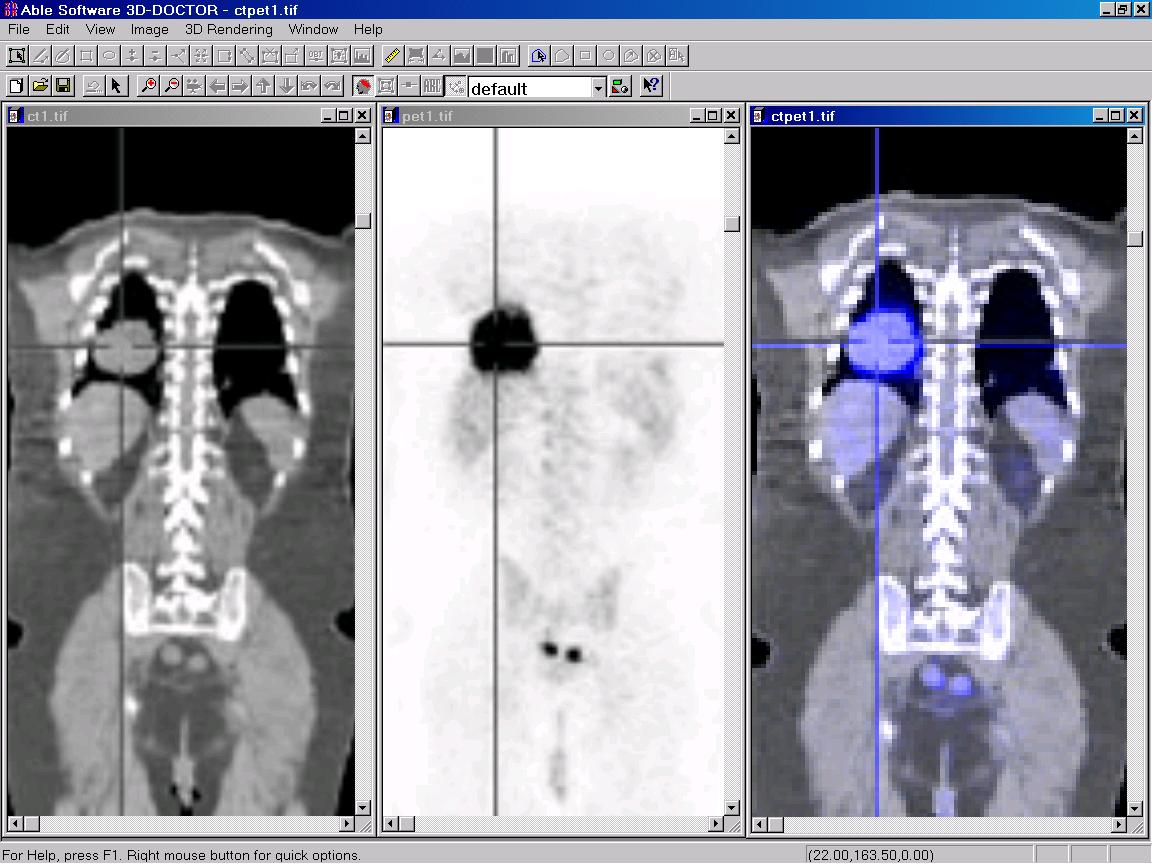
\includegraphics[scale= 0.5]{mul1.jpg}
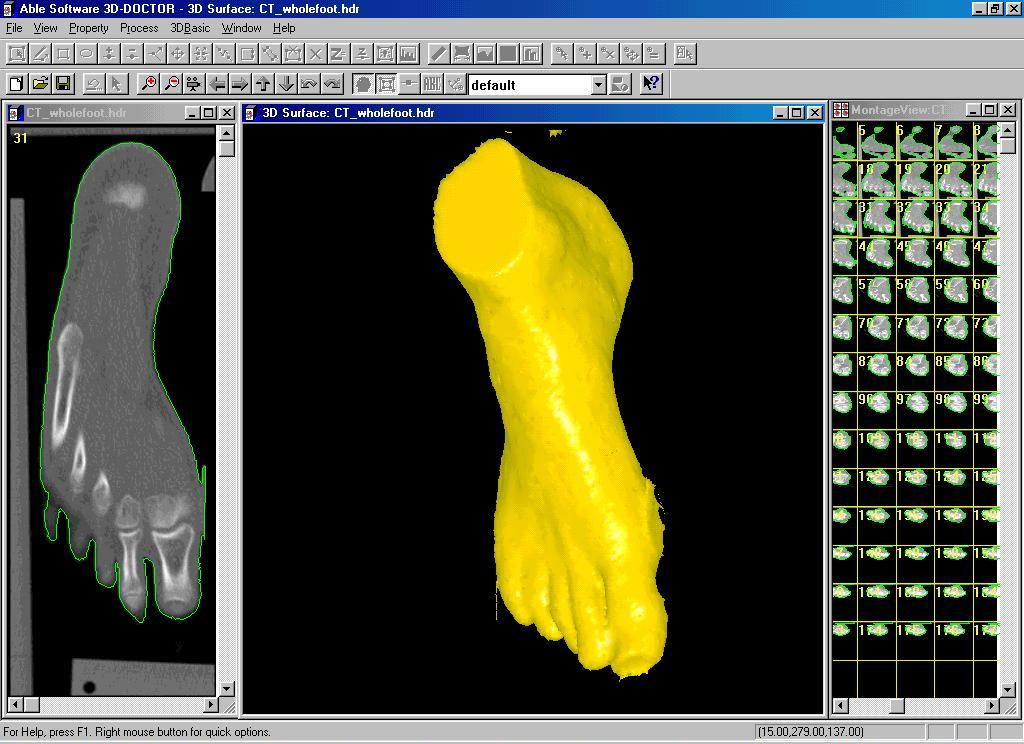
\includegraphics[scale= 0.5]{mul2.jpg}
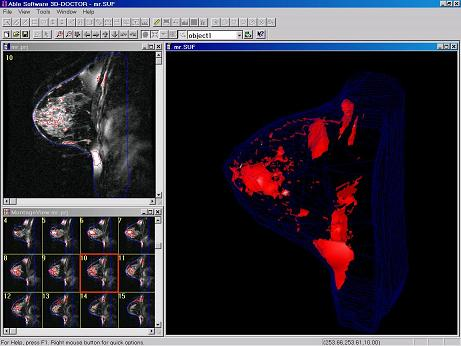
\includegraphics[scale= 0.7]{mul4.jpg}
\caption{Bone Modeling From CT  Scan}
\label{CT scan}
\end{figure}
\newpage
\section{Math Equation}
\subsection{Superscript}
$$3x^{34}-y^{10}+z^4=1$$
$$2x^{3x^{10}+9}+y^{100}=z^{x+1}$$
\subsection{Subscript}
$$9x_{34}-y_{98}+z_4=1$$
$$2x_{3a_{10}+9}+b_{100}=c_{x+1}$$
\subsection{Squrare Roots}
$$\sqrt[3]{x+4}=23$$     $$\sqrt[2]{a+b}+\sqrt[2]{x+5}=3$$
\subsection{Different types of Operators}
\begin{itemize}
\item[1.]
$\alpha-----A\alpha+x\beta=10\gamma$
\item[2.]
$\beta-----A\alpha+x\beta=10\gamma$
\item[3.]
$\gamma-----A\alpha+x\beta=10\gamma$
\item[4.]
$\pi-----\pi=3.14159399$
\item[5.]
$\log------\log_{10} ^{10}=1$
\item[6.]
$\ln------\ln(0)=0$
\item[7.]
$\sin$ ------- $\sin^2A+\cos^2A=1$
\end{itemize}
\subsection{Fraction}
$$\frac{3}{5}=\frac{x}{y}$$
$$\frac{a}{3}+\frac{b}{3}=\frac{x}{4}+\frac{y}{8}$$
\newpage

\section{Table}
\subsection{4 coloum 2 row table}
\begin{table}
\begin{tabular}{|l|l|l|l|}
\hline
x&y&z&1\\
\hline
1&3&4&8\\
\hline

\end{tabular}
\end{table}
\section{Reference}
\begin{itemize}
\item
google
\item
wikipedia
\item
youtube
\item
3D software demonstration by Dental Implant Specialist dental implants scarorough.

\end{itemize}
\end{document}
